\section{Deep Temporal Clustering}
\label{sec:DTC}
As already mentioned, the main problem that affects the \ac{AE} method in the \ac{SSE}-\ac{MSE} discrimination is related to the fact that a complex waveform with its own evolution in time is treated and calssified on the basis of a single number. This number should in principle be a simple summary of the behaviour of the signal, but actually does not account for the time evolution of it. This problem is still present in a certain way also in the \ac{VAE}-based classifier: even though we use 8 features (and not only one), these are striclty correlated with single physical quantities that could ideally be computed by hand. Therefore what is really needed is a deep learning model that collapses all dimensions but the temporal one. On top of that, a features extraction aimed at a classification task separates the two goals of getting a good reconstruction of the waveform, which means having learnt important features of it, from the clustering problem.

Madiraju et al. (2018) in their paper \textit{"Deep Temporal Clustering: fully unsupervised learning of time-domain features"} \cite{DTC} implemented an algorithm, called Deep Temporal Clustering, aimed at unsupervised clustering of time series data. Firstly an autoencoder is used to extract a latent-space representation in time of the input data and secondly a clustering algorithm assigns said latent representation to a time series prototype, i.e. the equivalent of a centroid in K-Means algorithms. A number of prototypes, equals to the number of clusters we need to identify, is predefined and then tuned during the clustering training in order to resemble a typical waveform of a given cluster. The power of this network lays in two specific aspects: first the fact that the time dimension is preserved also in the latent representation and second the fact that exploiting a combined optimisation of the two branches of the complexive model, i.e. the autoencoding and the clustering, spatio-temporal features are extracted in order to optimise the reconstruction \textit{and} the clustering simoultaneously. 
\subsection{Architecure} 
The \ac{DTC} algorithm implemented for this work follows the one of the original paper\footnote{The full code of the authors is available here: \url{https://github.com/FlorentF9/DeepTemporalClustering}.}, but introduces several modifications and improvements, most notably the transition from the original Keras implementation to PyTorch. The overall architecure can be decomposed into two main parts: the autoencoder, specifically called \ac{TAE}, and the clustering referred to as \ac{TSC}. 

\subsubsection{Temporal Autoencoder class}
The \ac{TAE} is an Autoencoder for which the latent space is given by a compacted time series which ideally represents the input and from which the latter can be reconstructed with the decoder.
The workflow of the \ac{TAE} follows this scheme:
\begin{itemize}
    \item \textbf{input waveforms}\\
    Input waveforms are current signals processed as explained above in Sec. \ref{sec:data-cleaning} with dimension ($1~\times~200$). The only difference with respect to the \ac{VAE} input is that in this case no \ac{SSE}/\ac{MSE} cut has been performed and the whole energy spectrum between $1550$ keV and $1650$ keV has been considered. 
    \item \textbf{temporal encoder}\\
    The temporal encoder is constructed as a sequential module \cite{torchSequential}
    \begin{enumerate}
        \item a 1D convolutional (\texttt{Conv1d}) layer with kernel size = 10, stride = 1 and padding = kernel size - 1 = 10 - 1 = 9\footnote{This is the default configuration of padding when stride = 1. This padding value will be the same in all convolutional layers of this class.}, mapping the ($1~\times~200$) input into a tensor with dimensions ($50~\times~200$);
        \item a LeakyReLU activation function, already detailed in Eq. \ref{eq:leakyReLU}, with $\alpha = 0.1$;
        \item a 1D max pooling layer (\texttt{MaxPool1d}) with kernel size = 10 returnin a ($50~\times~20$) object and thus significantly reducing the time dimensions; this first two layers, i.e. the convolutional and the pooling layers, are needed in order to obtain a more compact representation of time series: dimensionality reduction is needed for the following steps to avoid very long sequences that may lead to a bad performance.
        \item a bidirectional \ac{LSTM} (\texttt{LSTM}) receiving the 50 input features that uses 50 hidden units to return another ($50\times~20$) object. Specifically a \ac{LSTM} is used to learn temporal changes in both time directions. Since the standard PyTorch library does not natively implement the summation of the forward and backward outputs, a dedicated custom class was designed to perform this operation manually;
        \item a LeakyReLU activation function with $\alpha = 0.1$;
        \item another bidirectional \ac{LSTM} with only one hidden unit to compact features in a single tensor of dimensions ($1~\times~20$);
        \item a LeakyReLU activation function with $\alpha = 0.1$.
    \end{enumerate}
    \item \textbf{latent space}\\
    Differently respect to the \ac{VAE} case, the latent space is a compact time series with dimensions ($1~\times~20$), i.e. the output of the last layer of the encoder module. This representation maintains the sequential nature of input data but extract significant features that are indeed the output of both the decoder module and the clustering layer that will be discussed further in this Section.
    \item \textbf{temporal decoder}\\
    The decoder part tries to reconstruct the original waveform, starting from the latent-space small time series. In \cite{DTC} the decoder constited of a upsampling layer followed by a deconvolutional one. After preliminary trials where a very bad reconstruction was observed the following architecture has been preferred:
    \begin{enumerate}
        \item a 1D convolutional layer: 50 kernels of kernel size = 10, stride = 1 and padding = kernel size $-1$ = 10 $-1$ = 9 expands the ($1 \times 20$) object up to a ($50 \times 20$) dimensionality object, without changing the temporal resolution;
        \item a LeakyReLU activation is performed on the output of the previous layer with $\alpha = 0.1$;
        \item the ($50 \times 20$) object is upsampled in linear mode, with a scaling factor that returns a ($50 \times 200$) object;
        \item a 1D convolutional layer with kernel size = 10, stride = 1 and padding = kernel size $-1$ = 10 $-1$ = 9 maps the 50 features back to the original number of channels, that is exactly 1, giving the final ($1 \times 200$) reconstructed waveform.
    \end{enumerate}
    \item \textbf{output waveforms}\\
    Just as in the \ac{VAE} implementation, output waveforms are the latent-based reconstruction of input ones.
\end{itemize}

Although the original loss function used in \cite{DTC} was a Mean Square Error loss, this is not suitable for our signals, as already discussed in \ref{subsec:VAE-training}. Thus loss function that parametrises and corrects all of the just-mentioned steps of the \ac{TAE} part of \ac{DTC} is a \ac{NLL} as the one of Eq. \ref{eq:rec-loss}. Therefore the \ac{TAE} loss function results in Eq. \ref{eq:tae-loss}, where $\sigma$ is a trainable parameter of the model here as well as in the \ac{VAE} implementation. Specifically, this parameter is tuned in the initial part of the training, called \textit{pretrain}, where only the \ac{TAE} is used, and then fixed for the second part of the training where also the \ac{TSC} part is implemented. 
% The architecture can also be visualised in Fig.~\ref{fig:tae-architecure}.

\begin{equation}
    \label{eq:tae-loss}
    L_{\text{TAE}} = \frac{1}{B} \sum_{i=1}^{B} \left[ \frac{1}{2} \sum_{t=1}^{T} \left( \frac{\left( x_{i,t} - \hat{x}_{i,t} \right)^2}{\sigma^2} + \log \sigma^2 \right) \right]
\end{equation}

\begin{figure}[H]
    \centering
    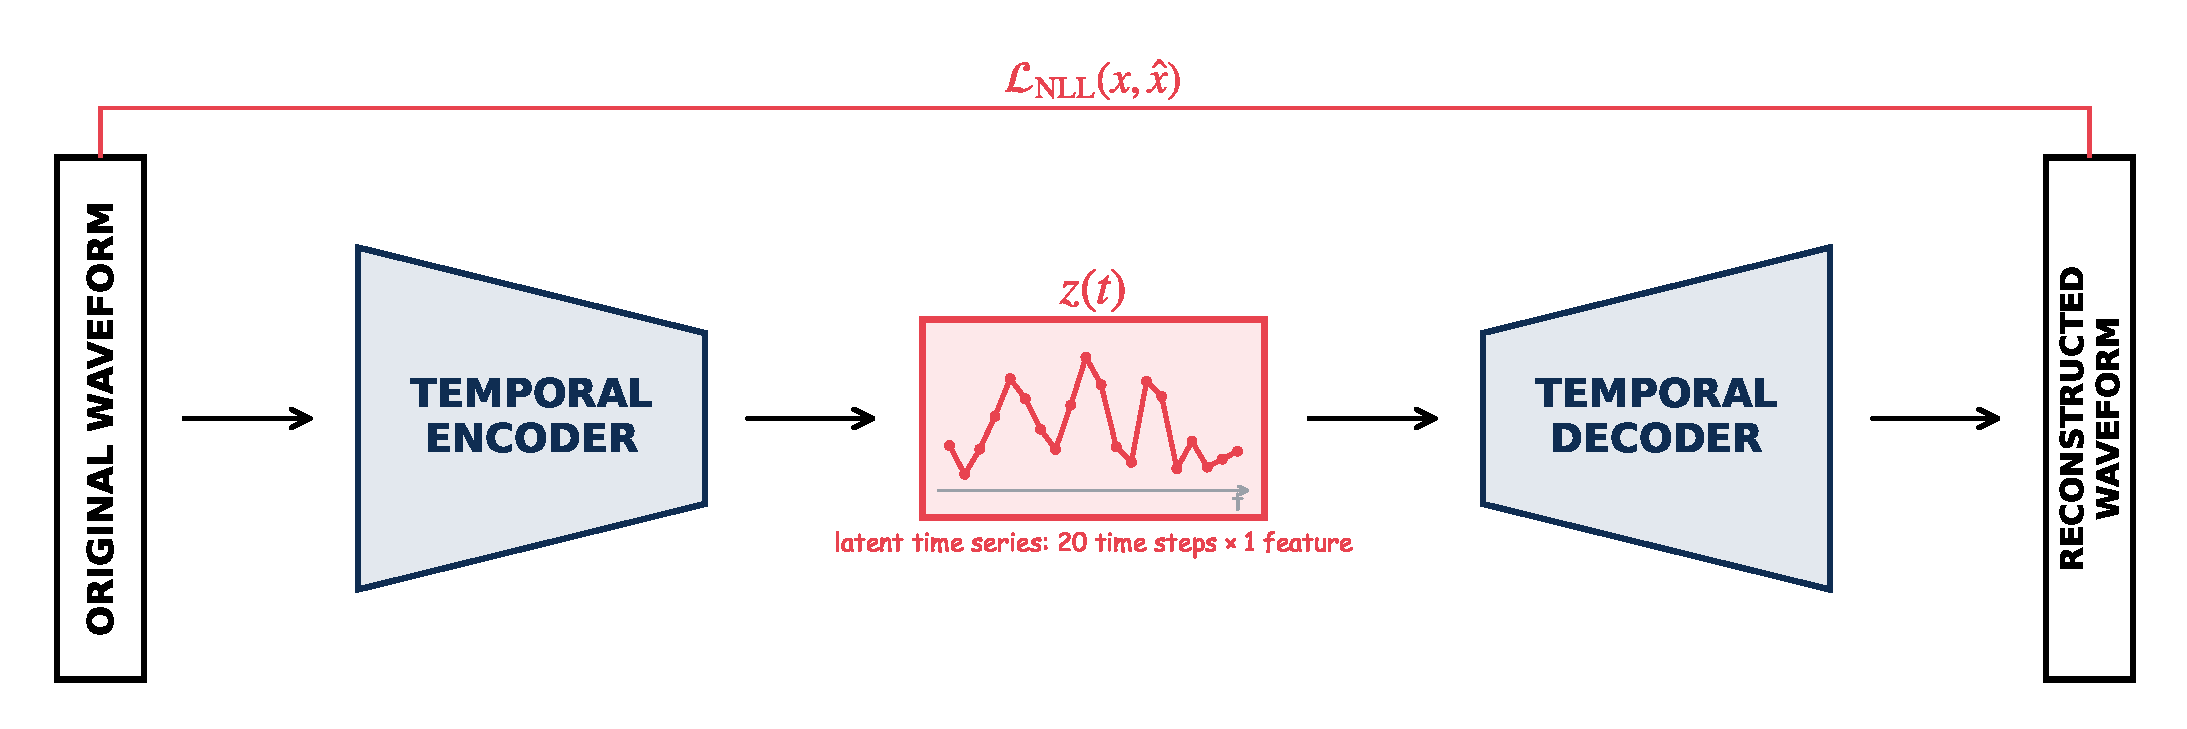
\includegraphics[width=\textwidth]{figures/schemi_output/TAE.pdf}
    \caption{Schematich representation of the \ac{TAE} architecture. The (temporal) endoer maps the input waveforms to a small time series in the latent space and the (temporal) decoder reconstruct waveforms from it. The model is mediated by a \ac{NLL} loss function.}
    \label{fig:tae-architecure}
\end{figure}

\subsubsection{Time Series Clustering class}
\label{subsubsec:TSC-class}
The \ac{TSC} class only consists of a tesorial object in the \texttt{Parameter} PyTorch class which represents the centroids for each class. Therefore this tensor parameter has dimensions (\texttt{clusters} $\times$ \texttt{length} $\times$ \texttt{features}) where the number of clusters is to be defined depending on how many different physical clusters we want to individuate and input length and channels are the ones of the latent representation of our input waveforms in the \ac{TAE}, in our case (\texttt{length} $\times$ \texttt{features}) = ($20~\times~1$). The cluster centroids tensor is first filled using the Xavier uniform initialisation \cite{Xavier}, which only acts as a placeholder: any non-constant initialisation breaks the symmetry between the centroids, whereas identical centroids would receive identical assignments ($q_{ij} = 1/k$) and zero gradients, and could never separate. Before the joint training, these values are overwritten by the centroids obtained by running KMeans on the latent representations of the training set, produced by the pre-trained \ac{TAE}\footnote{The original \ac{DTC} work uses hierarchical clustering with complete linkage for this step.}.
 The workflow of this class includes different steps:
\begin{itemize}
    \item \textbf{input acquisition}\\
    The clustering module receives the latent-space time sequences produced by the temporal encoder. Since standard 1D convolutional layers output tensors with dimensions ordered as (\texttt{features}~$\times$~\texttt{time steps}) = ($1~\times~20$), the latent tensor is first permuted to swap the channel and time axes. This yields a tensor with the expected shape of (\texttt{time steps}~$\times$~\texttt{features}) = ($20~\times~1$) in our setup. Finally, the permuted tensor is expanded along a new axis, preparing it for a broadcasted distance computation against all cluster centroids simultaneously, therefore obtaining ($1~\times~20\times~1$).
    \item \textbf{distance computation}\\
    A distance metric is computed between the input and each of the clusters centroids. Implemented metric distances are:
    \begin{itemize}
        \item \textbf{Euclidean Distance (EUC)}: given a latent sequence $x$ and a cluster centroid $w$, both made of $T$ time steps ($T = 20$, i.e. the input length divided by the pooling size), the distance is the usual geometrical distance of Eq. \ref{eq:EUC-distance}. Although it is the simplest and most intuitive metric, it compares the two sequences point by point, so it reacts to any difference in level, scale and timing between them. This is partly desirable, since the amplitude of the current carries the A/E information, but it also makes the metric sensitive to residual misalignments and noise, which can obscure the pulse-shape differences between SSE and MSE events\footnote{The alignment on the first current peak and the low-pass filter described in Sec. \ref{sec:data-cleaning} reduce these effects, but cannot remove them completely.}.
        \begin{equation}
            \label{eq:EUC-distance}
            d_\text{EUC}(x, w) = \sqrt{\sum_{t=1}^{T} (x_{t} - w_{t})^2}
        \end{equation}

        \item \textbf{Complexity-Invariant Distance (CID)}: this metric, introduced by Batista et al. \cite{Batista}, extends the Euclidean distance with a correction factor based on the complexity of the time series, which prevents two sequences with very different variability from being considered close. The complexity estimate $\mathrm{CE}$ of a series (Eq. \ref{eq:CE-factor}) is the norm of its discrete derivative, i.e. the square root of the sum of the squared differences between consecutive points. The final distance is the Euclidean distance multiplied by the ratio between the larger and the smaller complexity (Eq. \ref{eq:CID-distance}); this factor is always $\geq 1$ and equals 1 only when the two sequences have the same complexity.
        \begin{equation}
            \label{eq:CE-factor}
            \mathrm{CE}(x) = \sqrt{\sum_{t=1}^{T-1} (x_{t+1} - x_t)^2}
        \end{equation}
        \begin{equation}
            \label{eq:CID-distance}
            d_\text{CID}(x, w) = d_\text{EUC}(x, w) \cdot \frac{\max[\mathrm{CE}(x), \mathrm{CE}(w)]}{\min[\mathrm{CE}(x), \mathrm{CE}(w)]}
        \end{equation}

        \item \textbf{Auto-Correlation Function (ACF)}: this metric was introduced by Galeano \& Pe\~{n}a \cite{Galeano} and compares the latent sequence and the centroid through a weighted Euclidean distance between their autocorrelation coefficients. First, both sequences are converted into their sample autocorrelation functions $\varrho_x$ and $\varrho_w$ (Eq. \ref{eq:ACF}), computed for all the lags $k = 0, \dots, T-1$:
        \begin{equation}
            \label{eq:ACF}
            \varrho_x(k) = \frac{\sum_{t=1}^{T-k} (x_t - \bar{x})(x_{t+k} - \bar{x})}{\sum_{t=1}^{T} (x_t - \bar{x})^2}
        \end{equation}
        where $\bar{x}$ is the mean of the sequence. Since the mean is subtracted and the result is divided by the variance, $\varrho_x$ is invariant under any rescaling and shift of the latent sequence: it keeps only its temporal correlation structure, i.e. the width of the peaks and the separation between them, which shows up as a secondary bump of $\varrho_x$ at the corresponding lag. Second, a decaying diagonal matrix $\boldsymbol{\Omega}$ (Eq. \ref{eq:Omega-matrix}, with $m = T$) gives more weight to the lower lags: the coefficient at lag $k$ is estimated from only $T-k$ pairs of points, so the coefficients at high lags are the least reliable and are progressively suppressed.
        \begin{equation}
            \label{eq:Omega-matrix}
            \begin{aligned}
                \boldsymbol{\Omega} &= \begin{bmatrix} 
                \omega_0 & 0 & \cdots & 0 \\ 
                0 & \omega_1 & \cdots & 0 \\ 
                \vdots & \vdots & \ddots & \vdots \\ 
                0 & 0 & \cdots & \omega_{m-1} 
                \end{bmatrix} \\[1ex]
                \omega_k &= 1 - \frac{k}{m-1} \quad \text{for } k = 0, 1, \dots, m-1
            \end{aligned}
        \end{equation}
        Finally, the differences between the two autocorrelation functions are quantified as in Eq. \ref{eq:AC-distance}. Note that $\varrho(0) = 1$ for every sequence and $\omega_{m-1} = 0$, so neither the first nor the last lag contributes to the distance.
        \begin{equation}
            \label{eq:AC-distance}
            d_{\text{ACF}}(x, w) = \sqrt{(\varrho_x - \varrho_w)^{\top} \boldsymbol{\Omega} \, (\varrho_x - \varrho_w)}
        \end{equation}
    \end{itemize}
    \item \textbf{probability calculation}:\\
    The probability of belonging to a given cluster $j$ is based on a t-Student distribution kernel. Specifically, the similarity between the latent representation of a sample $x_i$ and a cluster centroid $w_j$ is evaluated using a Student's t-distribution with $\alpha$ degrees of freedom as a kernel. While the theoretical probability density function of the t-distribution includes a normalization constant defined by the Gamma function $\Gamma(\cdot)$, this term cancels out during the cluster assignment phase. In fact, to obtain valid soft assignments (i.e., probabilities that sum to 1), the score of cluster $j$ is normalized by the sum of the scores over all $k$ clusters \cite{DTC}. Since the degrees of freedom parameter $\alpha$ is a global constant across all clusters, the $\Gamma$ term simplifies algebraically, yielding the final probability $q_{ij}$ defined in Eq. \ref{eq:q-prob}:
    \begin{equation}
        \label{eq:q-prob}
        q_{ij} = \frac{\left( 1 + \frac{d(x_i, w_j)^2}{\alpha} \right)^{-\frac{\alpha+1}{2}}}{\sum_{k=1}^{K} \left( 1 + \frac{d(x_i, w_k)^2}{\alpha} \right)^{-\frac{\alpha+1}{2}}}
    \end{equation}
    where $d(x_i, w_j)$ is the distance metric chosen among the ones previously described, and $\alpha$ controls the heaviness of the distribution tails. From an architectural perspective, the heavy tails of the t-Student distribution are preferred over a standard Gaussian kernel because they prevent vanishing gradients for samples located far from the centroids, resulting in a more robust training process.
    \item \textbf{target distribution definition}:\\
    Being the \ac{DTC} a fully unsupervised method, a self-training mechanism is employed: seeing that the model doesn't have any target label, a target distribution built from $q_{ij}$ probabilities themselves is constructed, following the one in \cite{DTC}.
    Eq. \ref{eq:target-distribution-p} mathematically explains how said distribution is defined: Squaring $q_{ij}$ amplifies the most confident predictions, while $f_j$ (Eq.~\ref{eq:frequency-j}) is the soft frequency of cluster $j$, i.e. the sum of the assignment probabilities over the $B$ samples of the batch\footnote{In \cite{DTC} $f_j$ is computed over the whole dataset.}, so that dividing by it penalises very large clusters. The ratio $q^{2}_{ij}/f_j$ is then normalised over all the $K$ clusters.
    \begin{equation}
        \label{eq:target-distribution-p}
        p_{ij} = \frac{q^{2}_{ij} / f_j}{\sum_{k=1}^{K} q^{2}_{ik} / f_k}
    \end{equation}
    \begin{equation}
        \label{eq:frequency-j}
        f_j = \sum_{i=1}^{B} q_{ij}
    \end{equation}
\end{itemize}



Finally, the loss is computed as a \ac{KL} divergence, similar to the one used in Sec.~\ref{sec:vae-architeture}, averaged over the $B$ samples of a batch:

\begin{equation}
    \label{eq:KL-loss-TSC}
    L_{KL} = \frac{1}{B} \sum_{i=1}^{B} \sum_{j=1}^{K} p_{ij} \log \frac{p_{ij}}{q_{ij}}
\end{equation}

The target distribution is computed from the current $q_{ij}$ but it is treated as a constant, so that no gradient flows through it. Minimising Eq.~\ref{eq:KL-loss-TSC} therefore pushes $q_{ij}$ towards a sharper version of itself. Since $p_{ij}$ is recomputed at every update, the two distributions never simply coincide: as the assignments become more confident, so does the target, and the training converges towards high-confidence assignments.

Being \texttt{Parameter} objects, the centroids $w_j$ are optimised together with the weights of the \ac{TAE}, starting from the K-Means initialisation, by gradient descent on the total loss $L = L_\text{TAE} + \gamma \cdot L_{KL}$. However, seeing that $L_\text{TAE}$ does not depend on the centroids, they are moved only by the clustering term. For the Euclidean distance, $d_{ij}^2 = \lVert z_i - w_j \rVert^2$, the gradients are~\cite{KL-backpropagation}:

\begin{align}
    \frac{\partial L_{KL}}{\partial w_j} &= -\frac{\alpha+1}{\alpha B} \sum_{i=1}^{B} \left(1 + \frac{d_{ij}^2}{\alpha}\right)^{-1} (p_{ij} - q_{ij})\,(z_i - w_j) \label{eq:grad-centroids} \\
    \frac{\partial L_{KL}}{\partial z_i} &= \frac{\alpha+1}{\alpha B} \sum_{j=1}^{K} \left(1 + \frac{d_{ij}^2}{\alpha}\right)^{-1} (p_{ij} - q_{ij})\,(z_i - w_j) \label{eq:grad-latent}
\end{align}

Eq.~\ref{eq:grad-centroids} has an intuitive interpretation: if the target assigns sample $i$ to cluster $j$ with more confidence than the model ($p_{ij} > q_{ij}$), the gradient step moves the centroid $w_j$ towards $z_i$, while if $p_{ij} < q_{ij}$ it moves it away. The factor $(1 + d_{ij}^2/\alpha)^{-1}$ gives more weight to the samples that are already close to the centroid. At the same time, Eq.~\ref{eq:grad-latent} is back-propagated through the encoder, so that the latent representation $z_i$ of each sample is pulled towards the centroid of the cluster it most likely belongs to: the clustering reshapes the latent space itself, while $L_{NLL}$ keeps it faithful to the input waveforms. For the Complexity-Invarian Distance and the Autocorrelation Function the gradients follow from the same chain rule and are computed by automatic differentiation.


The full \ac{DTC} model that includes both the \ac{TAE} and the \ac{TSC} is shown in Fig.~\ref{fig:tae_and_tsc-architecure}.
\begin{figure}[H]
    \centering
    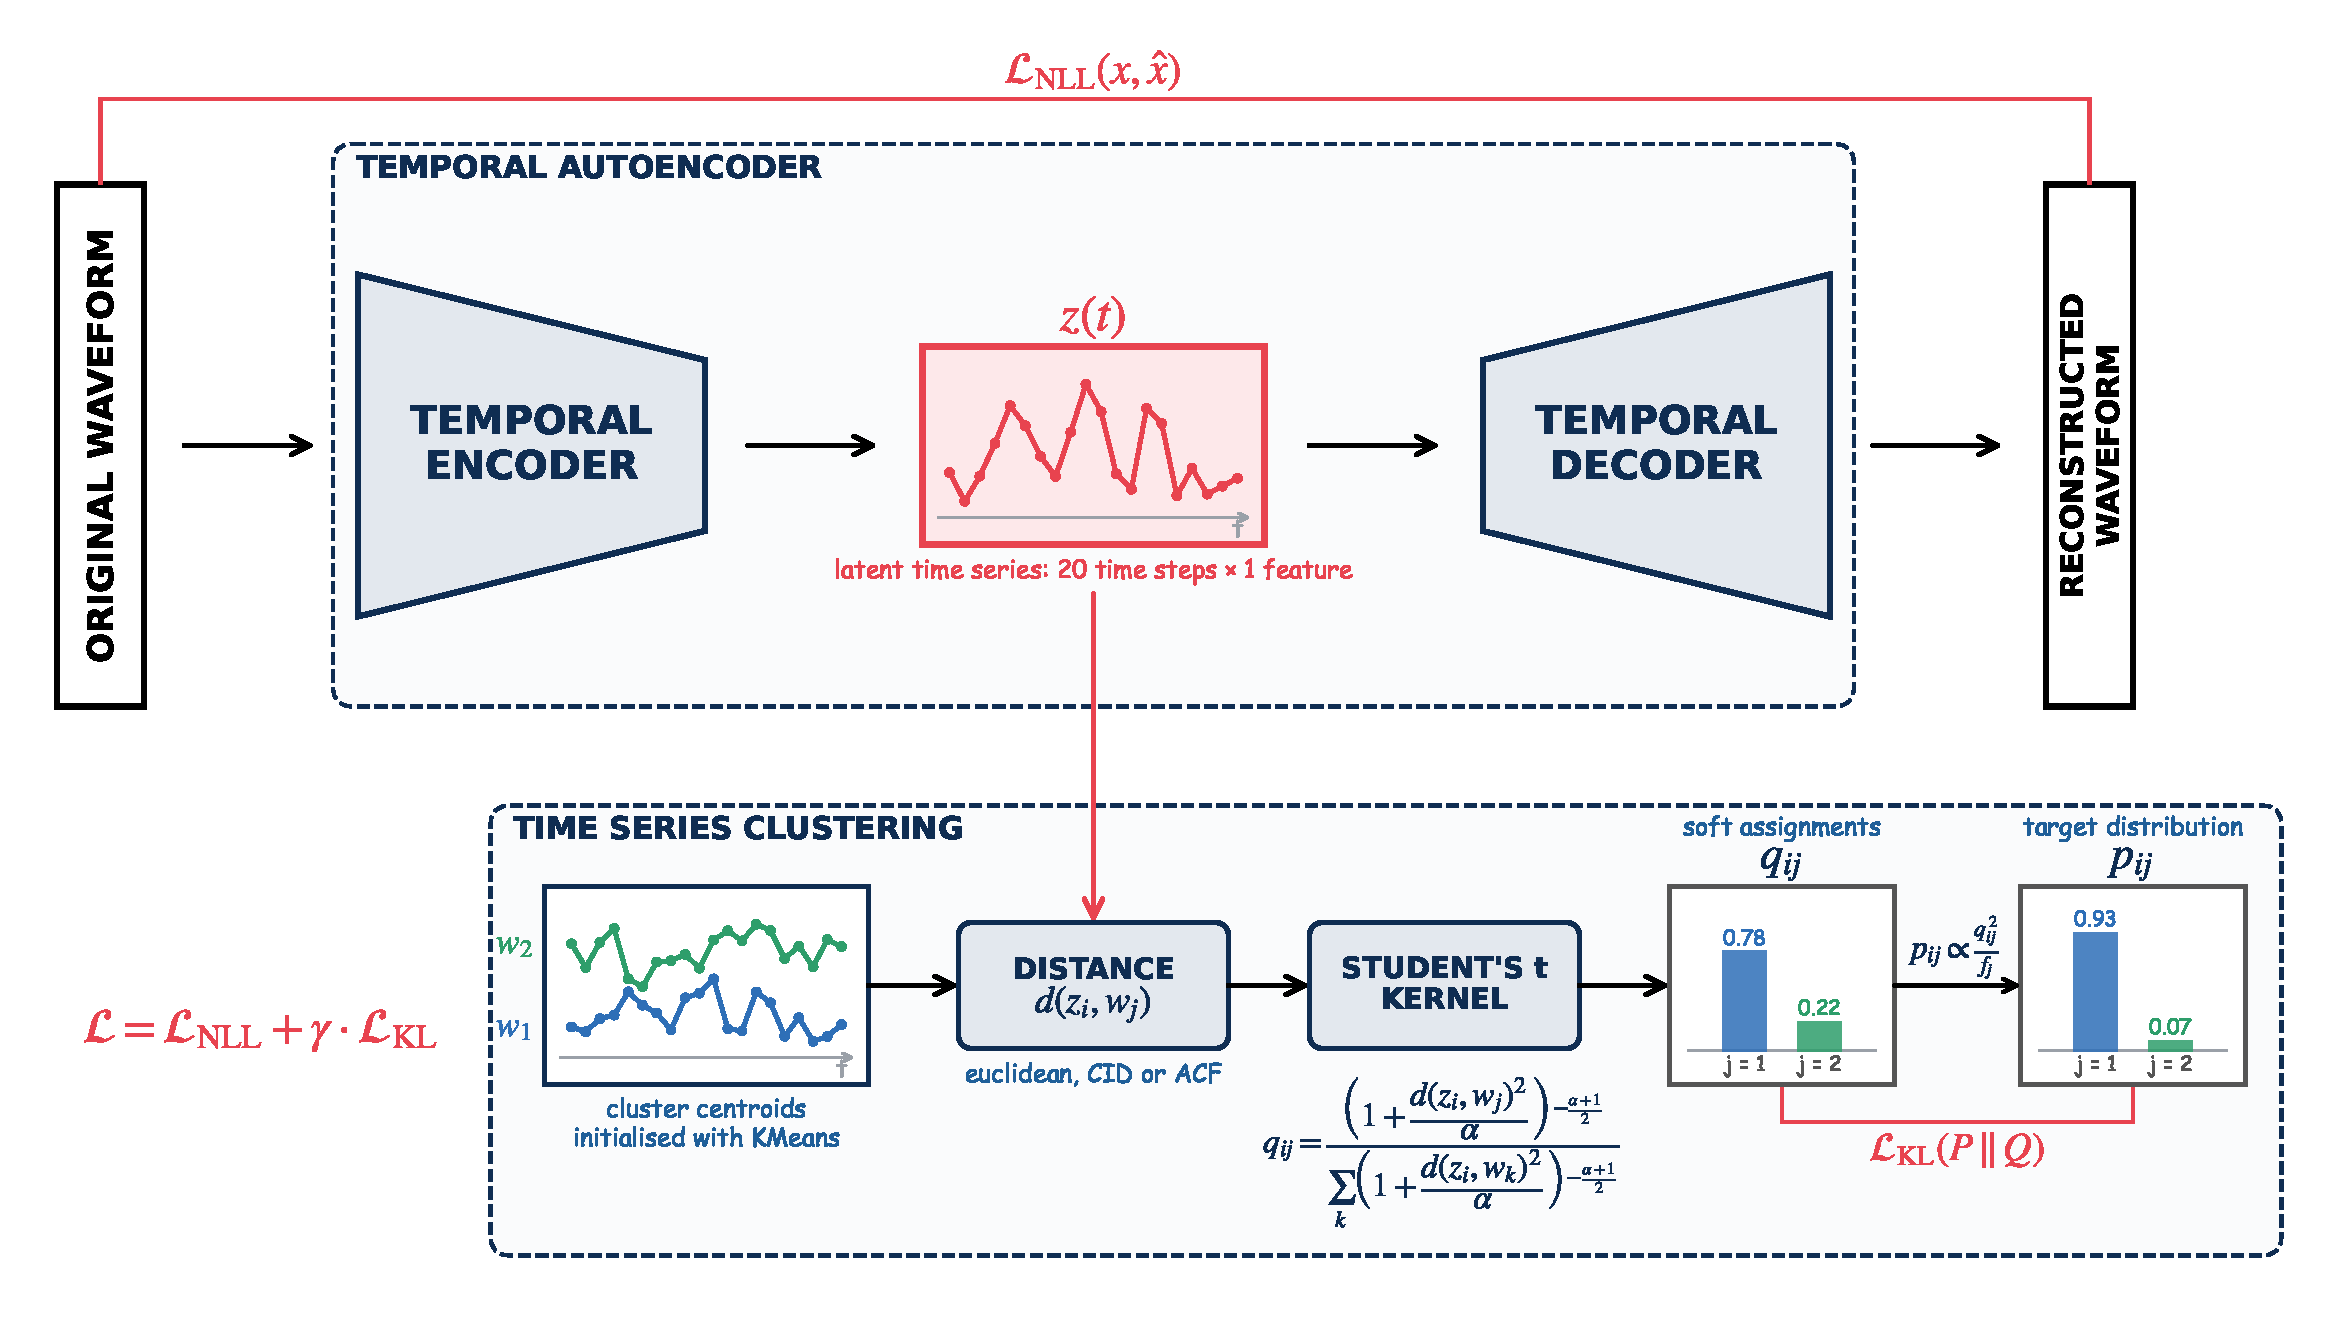
\includegraphics[width=\textwidth]{figures/schemi_output/TAE_clustering.pdf}
    \caption{Schematich representation of the \ac{DTC} architecture. The (temporal) encoder maps the input waveforms to a small time series in the latent space and the (temporal) decoder reconstruct waveforms from it. Moreover the time-series latent space is used to separate waveforms in different clusters. The full model is mediated by the \ac{NLL} loss function for the \ac{TAE} and the \ac{KL} divergence for the \ac{TSC}.}
    \label{fig:tae_and_tsc-architecure}
\end{figure}


\subsection{Data selection}
Being a fully-unsupervised clustering algorithm, the \ac{DTC} model does not require a specific data selection before its training. Therefore all the events in the 1550-1650 keV range of the calibration dataset, i.e. the whole gray spectrum of Fig.~\ref{fig:distribution-AoE_prl25}, have been employed as input waveforms of this algorithm, for a total $N_\text{DTC} = 348 999$ waveforms divided in the training, validation and test set as detailed in Table \ref{tab:sets-DTC}.
\begin{table}[H]
    \centering
    \begin{tabular}{cc}
        \toprule
        set & number of waveforms\\
        \midrule
        training & 279 199 \\
        validation & 34 900 \\
        test & 34 900\\
        \bottomrule
    \end{tabular}
    \caption{Division of events between the training, validation and test sets for the \ac{DTC} model.}
    \label{tab:sets-DTC}
\end{table}

The validation set has been used in this model, as well as in the previous one, to make sure the model does not overfit and to monitor that both the training and validation loss are decreasing through epochs.


\subsection{Training and testing}
The \ac{DTC} training phase is divided in two different parts: the \textit{pretrain}, where only the \ac{TAE} is used and then the proper \textit{train} where both the \ac{TAE} and the \ac{TSC} are implemented. 

\textbf{\textit{Pretrain}}: this phase is used in order to make the model learning how to reconstruct the input waveforms from the latent representation, without being affected by the clustering algorithm. The loss function used is the one described in Eq. \ref{eq:tae-loss} and as already introduced the parameter $\sigma$ in this phase is a learnable parameter on which the backpropagation acts. The model is trained for a number of epochs $\text{N}_\text{PRE} = 40$. The reconstruction ability of the \ac{TAE} is shown in Fig. \ref{fig:pretrain-validation} for a waveform in the validation set at different epochs. Fig. \ref{fig:pretrain-loss} shows the \ac{NLL} loss evolution: it is evident that both the training set loss and the validation one decreases over time, ensuring the fact that the model is actually learning how to recontruct waveforms and it is not overfitting training data.
\begin{figure}[H]
    \centering
    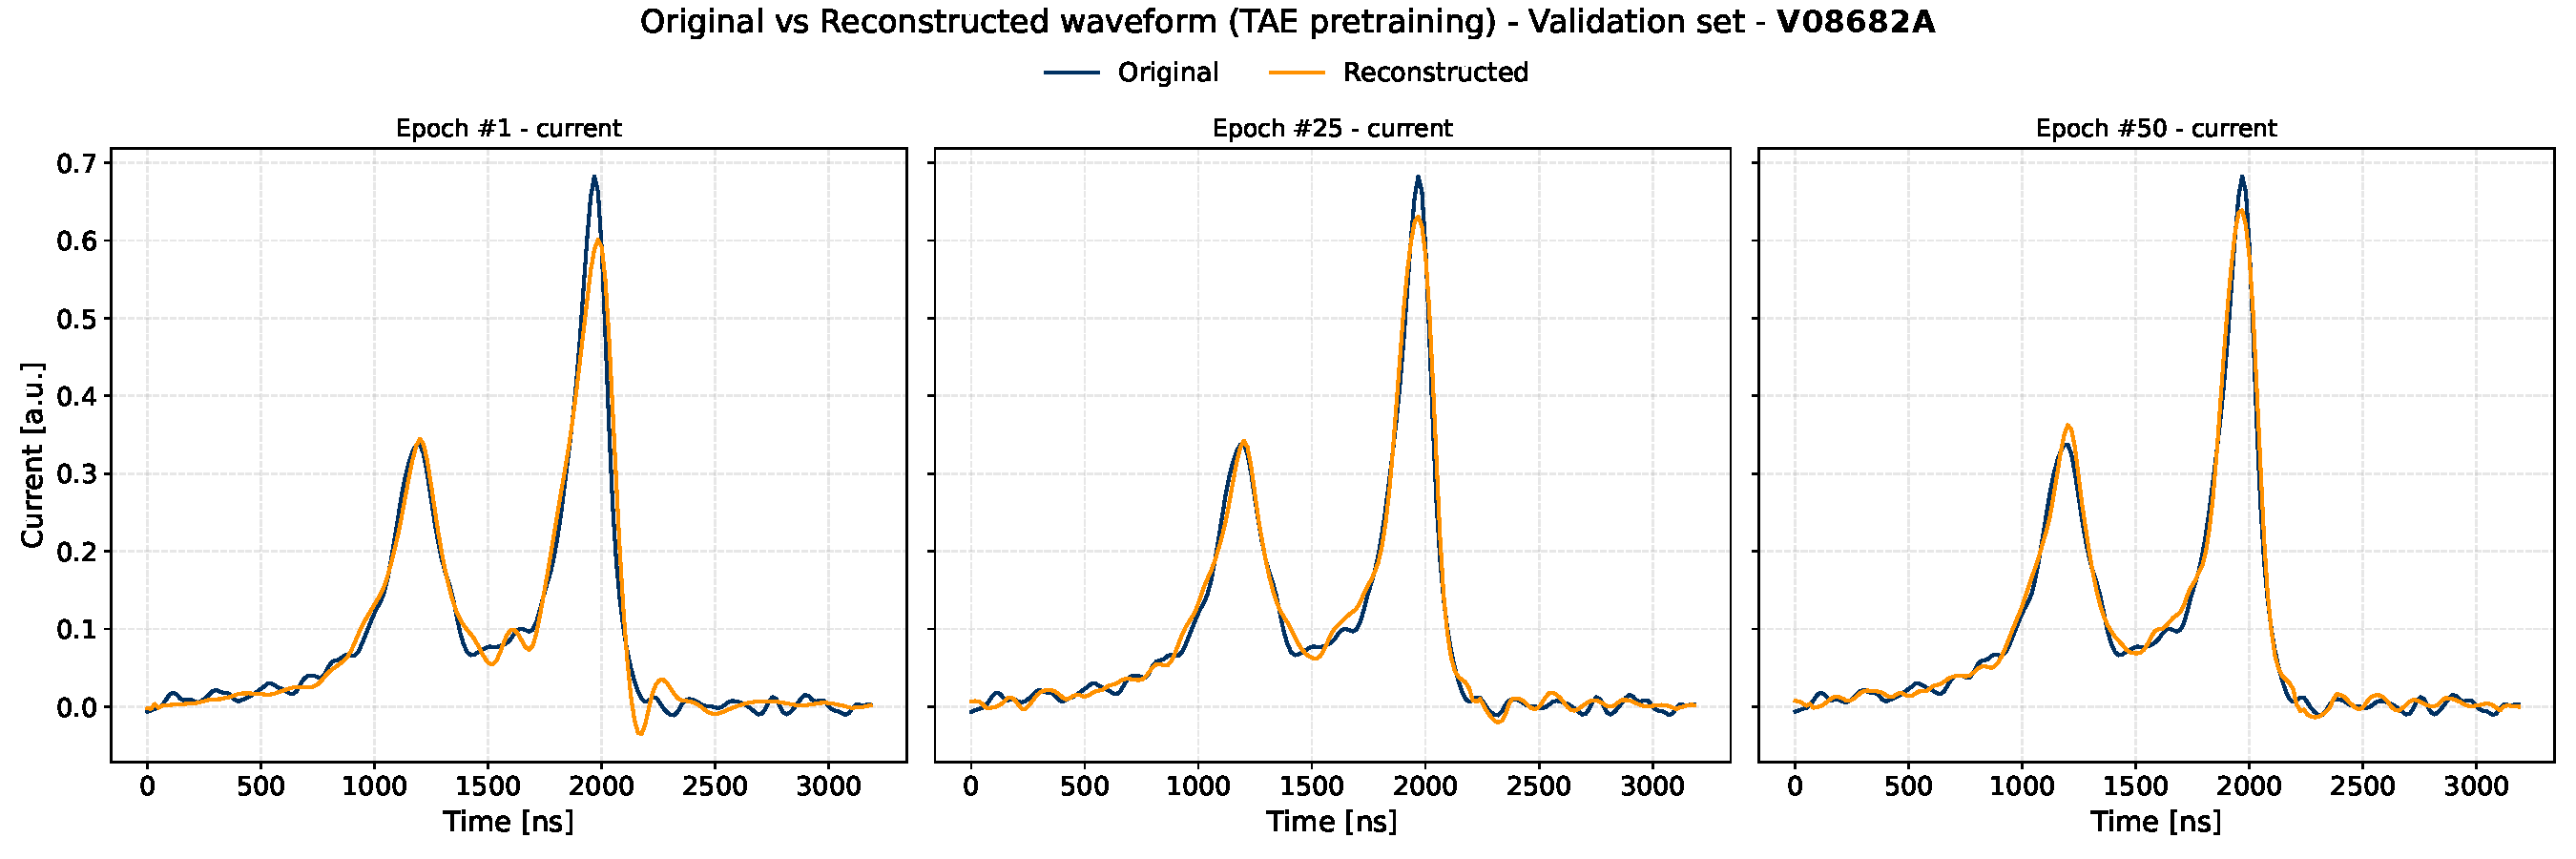
\includegraphics[width=\textwidth]{plots/DTC/pretrain_reconstruction.pdf}
    \caption{Example of the \ac{TAE} reconstruction ability in the \textit{pretrain} for a validation set waveform at epoch 1, 20, 40.}
    \label{fig:pretrain-validation}
\end{figure}

\begin{figure}[H]
    \centering
    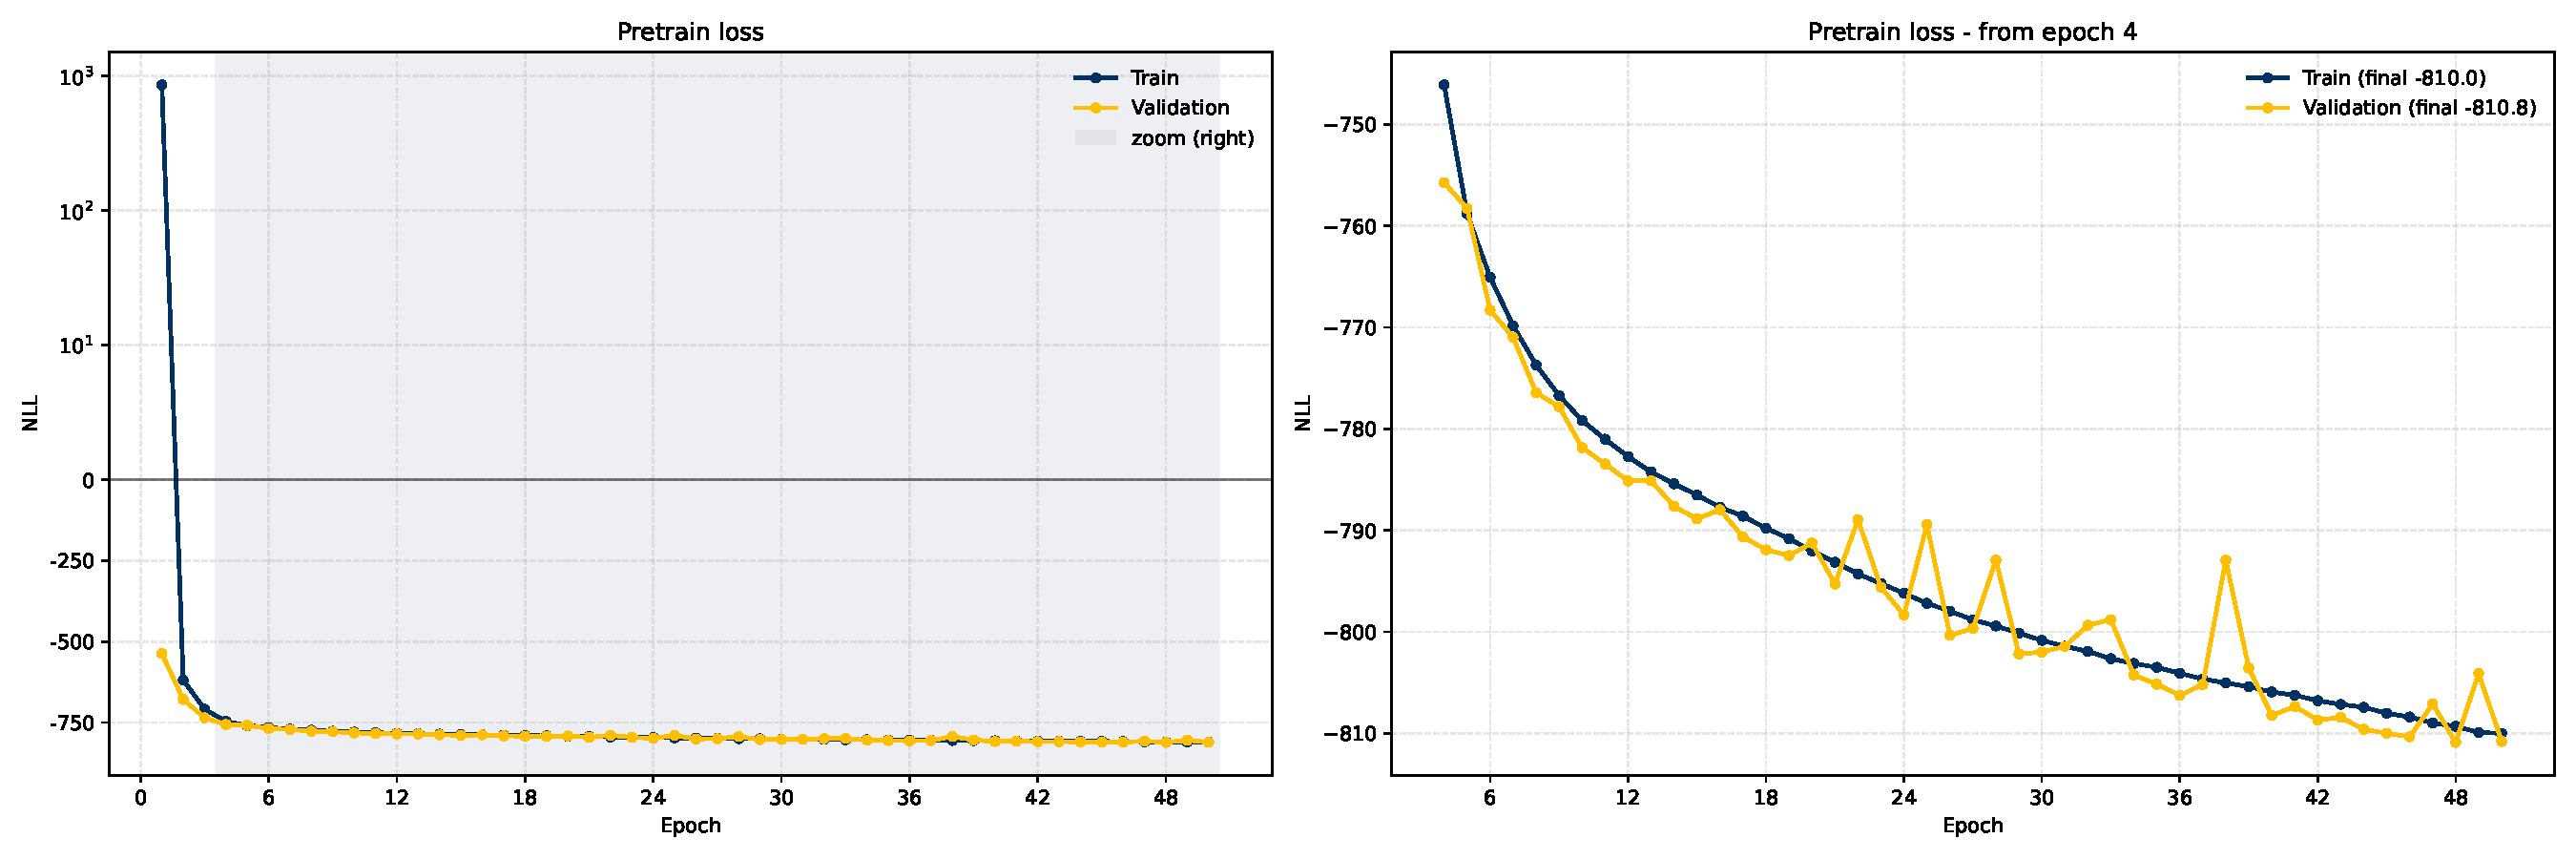
\includegraphics[width=\textwidth]{plots/DTC/pretrain_losses.pdf}
    \caption{\textit{Pretrain} loss evolution through epochs. On the right a zoom of the grey part of the left plot is shown.}
    \label{fig:pretrain-loss}
\end{figure}

Soon after this part is completed, the $\sigma$ parameter is fixed to the learned value and the centroids of the clusters are pre-initialised using a K-Means algorithm on the latent representation of the training set. It is from said centroids that the \ac{TSC} part of the mdoel starts to cluster waveforms.

\textbf{\textit{Train}}: in the second phase of the \ac{DTC} training, the proper \textit{training} phase, both the \ac{TAE} and the \ac{TSC} are used. As a consequence, the complexive loss function includes $L_\text{TAE}$ and $L_\text{TSC}$, weighted by a specific tunable parameter $\gamma$ in order to have the total loss of Eq. \ref{eq:total_dtc_loss}. Therefore the backpropagation acts both on the reconstruction of input waveforms and on the clustering of them simultaneously.
\begin{equation}
    \label{eq:total_dtc_loss}
    L_\text{DTC} = L_\text{TAE} + \gamma \cdot L_\text{TSC}
\end{equation}

The results of the complexive training part with $\text{N}_\text{TRAIN} = 20$ epochs and $\gamma = 1000$ are shown in Fig. \ref{fig:training-reconstruction-DTC}and \ref{fig:training-clustering-DTC} for the reconstruction and clustering part respectively and for all of the abovementioned distance metrics.
\begin{figure}[H]
    \centering
    
\includegraphics[width=0.5\textwidth]{plots/placeholder.png}
    \caption{\colorbox{yellow}{PLACEHOLDER}}
    \label{fig:training-reconstruction-DTC}
\end{figure}

\begin{figure}[H]
    \centering
    
\includegraphics[width=0.5\textwidth]{plots/placeholder.png}
    \caption{\colorbox{yellow}{PLACEHOLDER}}
    \label{fig:training-clustering-DTC}
\end{figure}


